A Digital Twin (DT) is formally defined as a digital representation of a physical item or assembly, using integrated simulations and service data. Designed to predict current and future conditions in both design and operational environments to improve decision-making, the digital representation integrates information from multiple sources throughout the product life cycle and is continuously updated \citep{fuller2020, jiang2021}.

The fundamental characteristic of DT is the level of data integration, classifying the models into three levels: (a) Digital model: it is a digital version of a physical object where there is no automatic switching between the physical model and the digital model; (b) Digital shadow: it has a unidirectional data flow, and therefore, changes to a physical object automatically change the digital object, but the reverse is not true; and (c) Digital Twin: it is defined by the complete integration of data flow in both directions \citep{iranshahi2025digital}.

Table \ref{tab:digital_capabilities} presents a consolidated overview of the capabilities and progression levels associated with Digital Models, Digital Shadows, and Digital Twins. As illustrated in Figure \ref{fig:dt_levels}, these three paradigms differ fundamentally in terms of data integration, automation maturity, and real-time interaction between physical and digital assets.

\begin{table}[htbp!]
\centering
\caption{Comparing the capabilities of Digital Twins, Digital Shadows, and Digital Models in performing different functions \citep{iranshahi2025digital}.}
\label{tab:digital_capabilities}
\begin{tabular}{p{7cm}ccc}
\toprule
\textbf{Functions} & \textbf{Digital Model} & \textbf{Digital Shadow} & \textbf{Digital Twin} \\
\midrule
Automatic data flow; from physical object to digital model. & $\times$ & $\checkmark$ & $\checkmark$ \\
Automatic data flow; from digital model to physical object. & $\times$ & $\times$ & $\checkmark$ \\
Predictive analysis; Testing scenarios virtually before applying them physically. & $\checkmark$ & $\checkmark$ & $\checkmark$ \\
Real-time monitoring of its real-world counterpart. & $\times$ & $\checkmark$ & $\checkmark$ \\
Decision-making; Real-time data analysis and predictive evaluation. & $\checkmark$ & $\checkmark$ & $\checkmark$ \\
Control; Real-time interaction and optimization of the physical system. & $\times$ & $\times$ & $\checkmark$ \\
\bottomrule
\end{tabular}
\end{table}


\begin{figure}[htbp!]
\centering
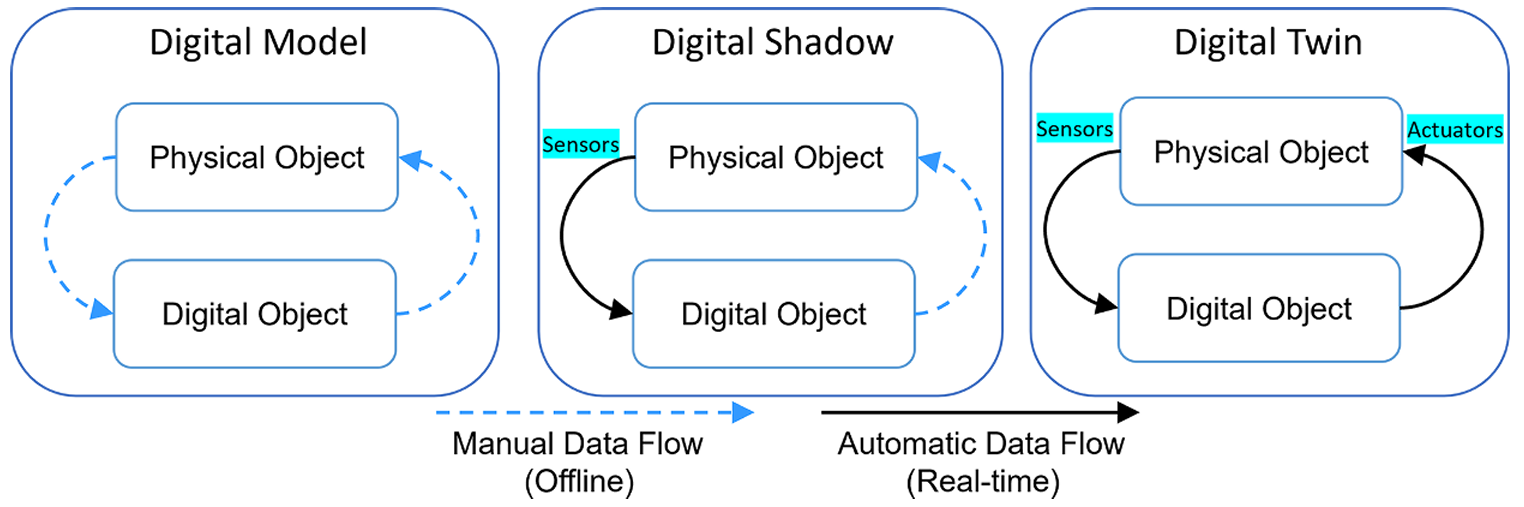
\includegraphics[width=0.85\textwidth]{z_fig_dt_level.png}
\caption{Conceptual differentiation among Digital Model, Digital Shadow, and Digital Twin based on data-flow direction and automation level \parencite{iranshahi2025digital}.}
\label{fig:dt_levels}
\end{figure}


